
\documentclass{beamer}
%
\usepackage{beamerthemesplit}
\usepackage{cite}
\usepackage{graphicx,epspdfconversion}
\usepackage{times}
\usepackage{amsmath,amsfonts,amssymb}
\usepackage{psfrag,latexsym,stmaryrd,color,bbm,mathrsfs}
%\mode<presentation> { \usetheme{Warsaw} }

\usetheme{Darmstadt}
%\usefonttheme[onlylarge]{structurebold}
\setbeamerfont*{frametitle}{size=\normalsize,series=\bfseries}
\setbeamertemplate{navigation symbols}{}

%
\title{Function Classification \\with Neural Networks}
\author{Pascal S.P. Steger}
\date[10. 08. 2010]{Theory, Simulation, Programming of Neural Networks, 2010}
%
%\pgfdeclaremask{eth}{ethlogo_kurz}
\pgfdeclareimage[width=1cm]{fig/ethlogo_kurz}{fig/ethlogo_kurz}
%
\logo{\pgfuseimage{fig/ethlogo_kurz}}
% 
\begin{document}
%
\begin{frame}
    \titlepage
\end{frame}
%
%
\section{Introduction}
%
%\subsection{overview}
\begin{frame}
    \tableofcontents
\end{frame}
%
\begin{frame}
\frametitle{Literature}
    \bibliographystyle{plain}
    \bibliography{qc_bib}
    % in order to display all literature: reference articles, books
	% shows up as [1] [2] [3] [4]
	\hfill\vfill
	\cite{Stoop2010}
	\cite{Rojas1996}
	\cite{Laemmel2004}
	\cite{Jones1990}
\end{frame}
%

\subsection{Neural Network: Topology}
\begin{frame}
%\frametitle{Topology}
	\begin{figure}
		\centering
		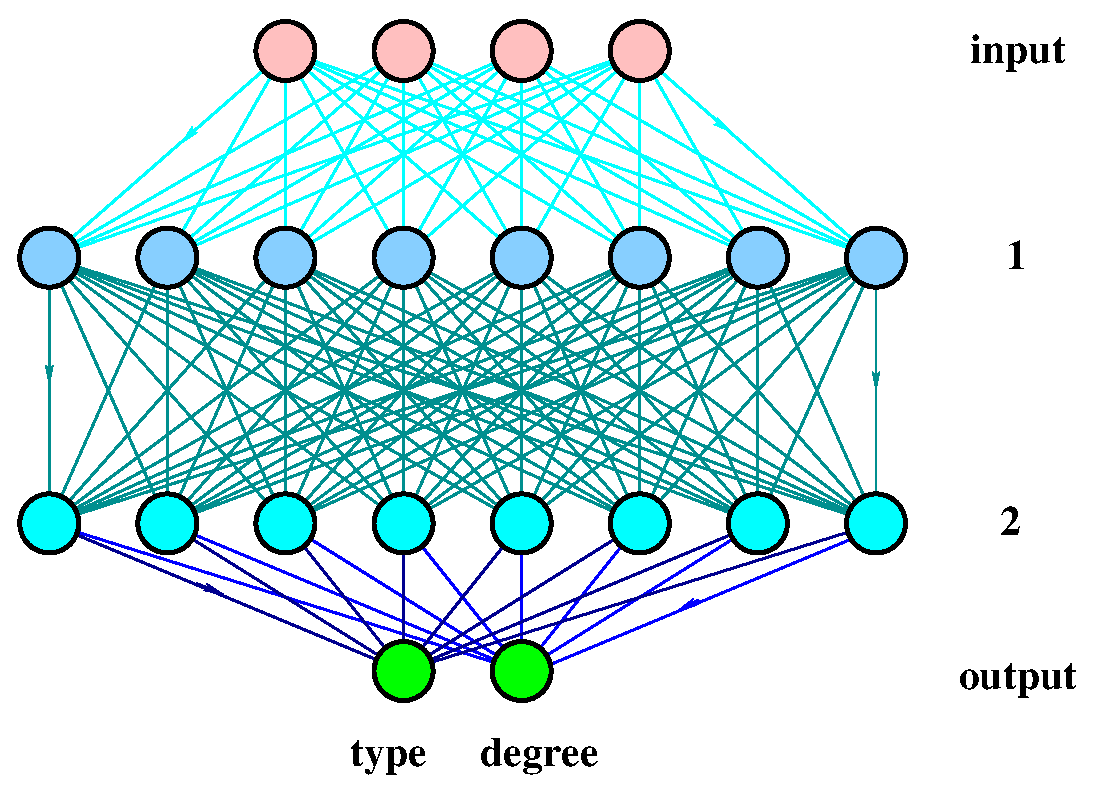
\includegraphics[width=6.5cm]{fig/network_topology.eps}
	\end{figure}
\end{frame}

\subsection{Backpropagation}
\begin{frame}
%\frametitle{Backpropagation}
\begin{table}
\begin{tabular}{lcl}

\texttt{ohh}&\texttt{=} &\texttt{sigmoid[whh.in];}\\
\texttt{oh} &\texttt{=} &\texttt{sigmoid[wh.ohh];}\\
\texttt{out}&\texttt{=} &\texttt{sigmoid[wo.oh];}\\
&&\\
\texttt{e}  &\texttt{=} &\texttt{t - out;}\\
\texttt{od} &\texttt{=} &\texttt{e out (1 - out);}\\
\texttt{hd} &\texttt{=} &\texttt{oh (1 - oh) [wo'].od;}\\
\texttt{hhd}&\texttt{=} &\texttt{ohh (1 - ohh) [wh'].hd;}\\
&&\\
\texttt{wo} &\texttt{+=}&\texttt{eta Outer[Times, od, oh];}\\
\texttt{wh} &\texttt{+=}&\texttt{eta Outer[Times, hd, ohh];}\\
\texttt{whh}&\texttt{+=}&\texttt{eta Outer[Times, hhd, in];}
\end{tabular}
\end{table}

\end{frame}



\section{Methods}
% \subsection{overview}
\begin{frame}
  \tableofcontents
\end{frame}

\subsection{Functions}
\begin{frame}
%  \frametitle{Function Classes}
  \begin{figure}
    \centering
    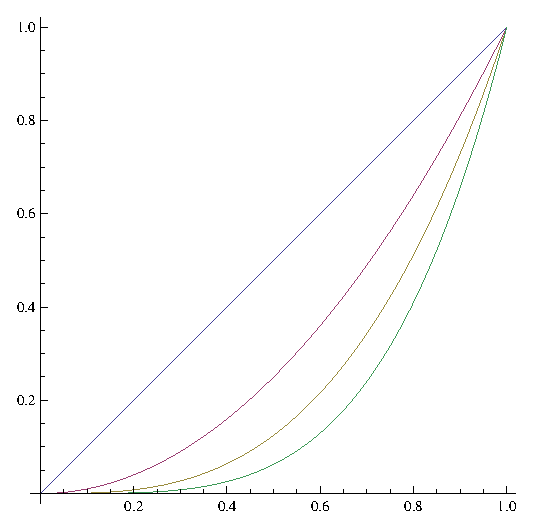
\includegraphics[width=2.5cm]{fig/Template1n.eps}
    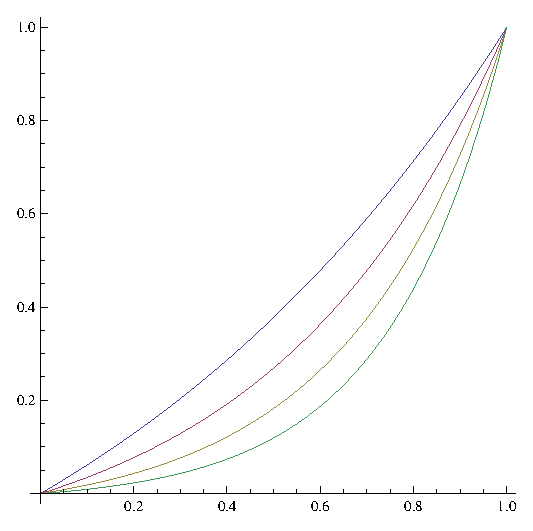
\includegraphics[width=2.5cm]{fig/Template2n.eps}
    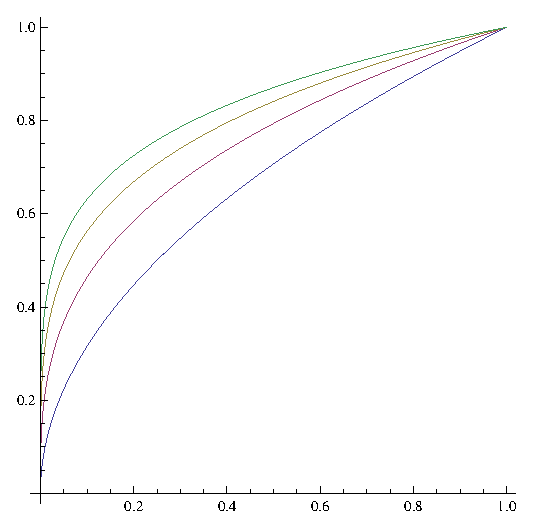
\includegraphics[width=2.5cm]{fig/Template3n.eps}
  \end{figure}
  \begin{equation*}
    x^n\qquad\qquad\exp(nx)\qquad\qquad x^{1/(1+n)}
  \end{equation*}
  \begin{figure}
    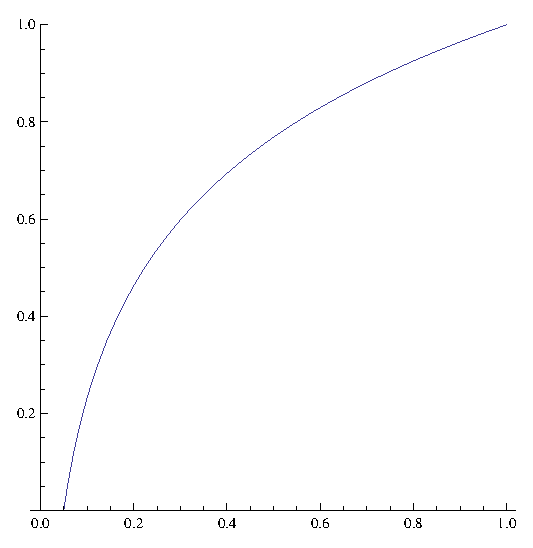
\includegraphics[width=2.5cm]{fig/Template4n.eps}
    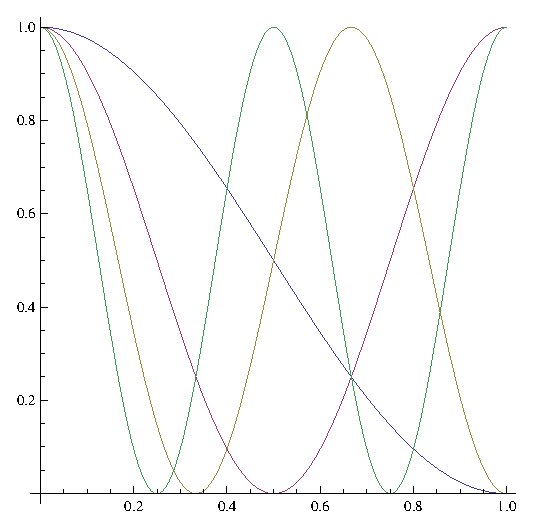
\includegraphics[width=2.5cm]{fig/Template5n.eps}
    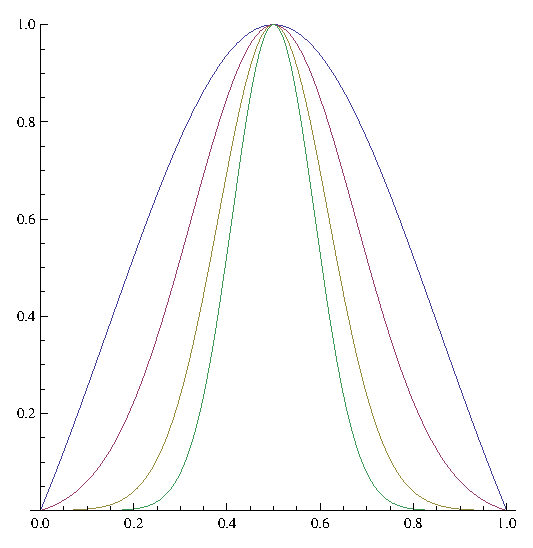
\includegraphics[width=2.5cm]{fig/Template6n.eps}
  \end{figure}
  \begin{equation*}
    \qquad\qquad\log(nx)\qquad\qquad\cos(n\pi x)\qquad e^{(-(2n(x-0.5))^2)}\qquad
  \end{equation*}
\end{frame}

\subsection{Program Flux}
\begin{frame}
  \begin{figure}
    \centering
    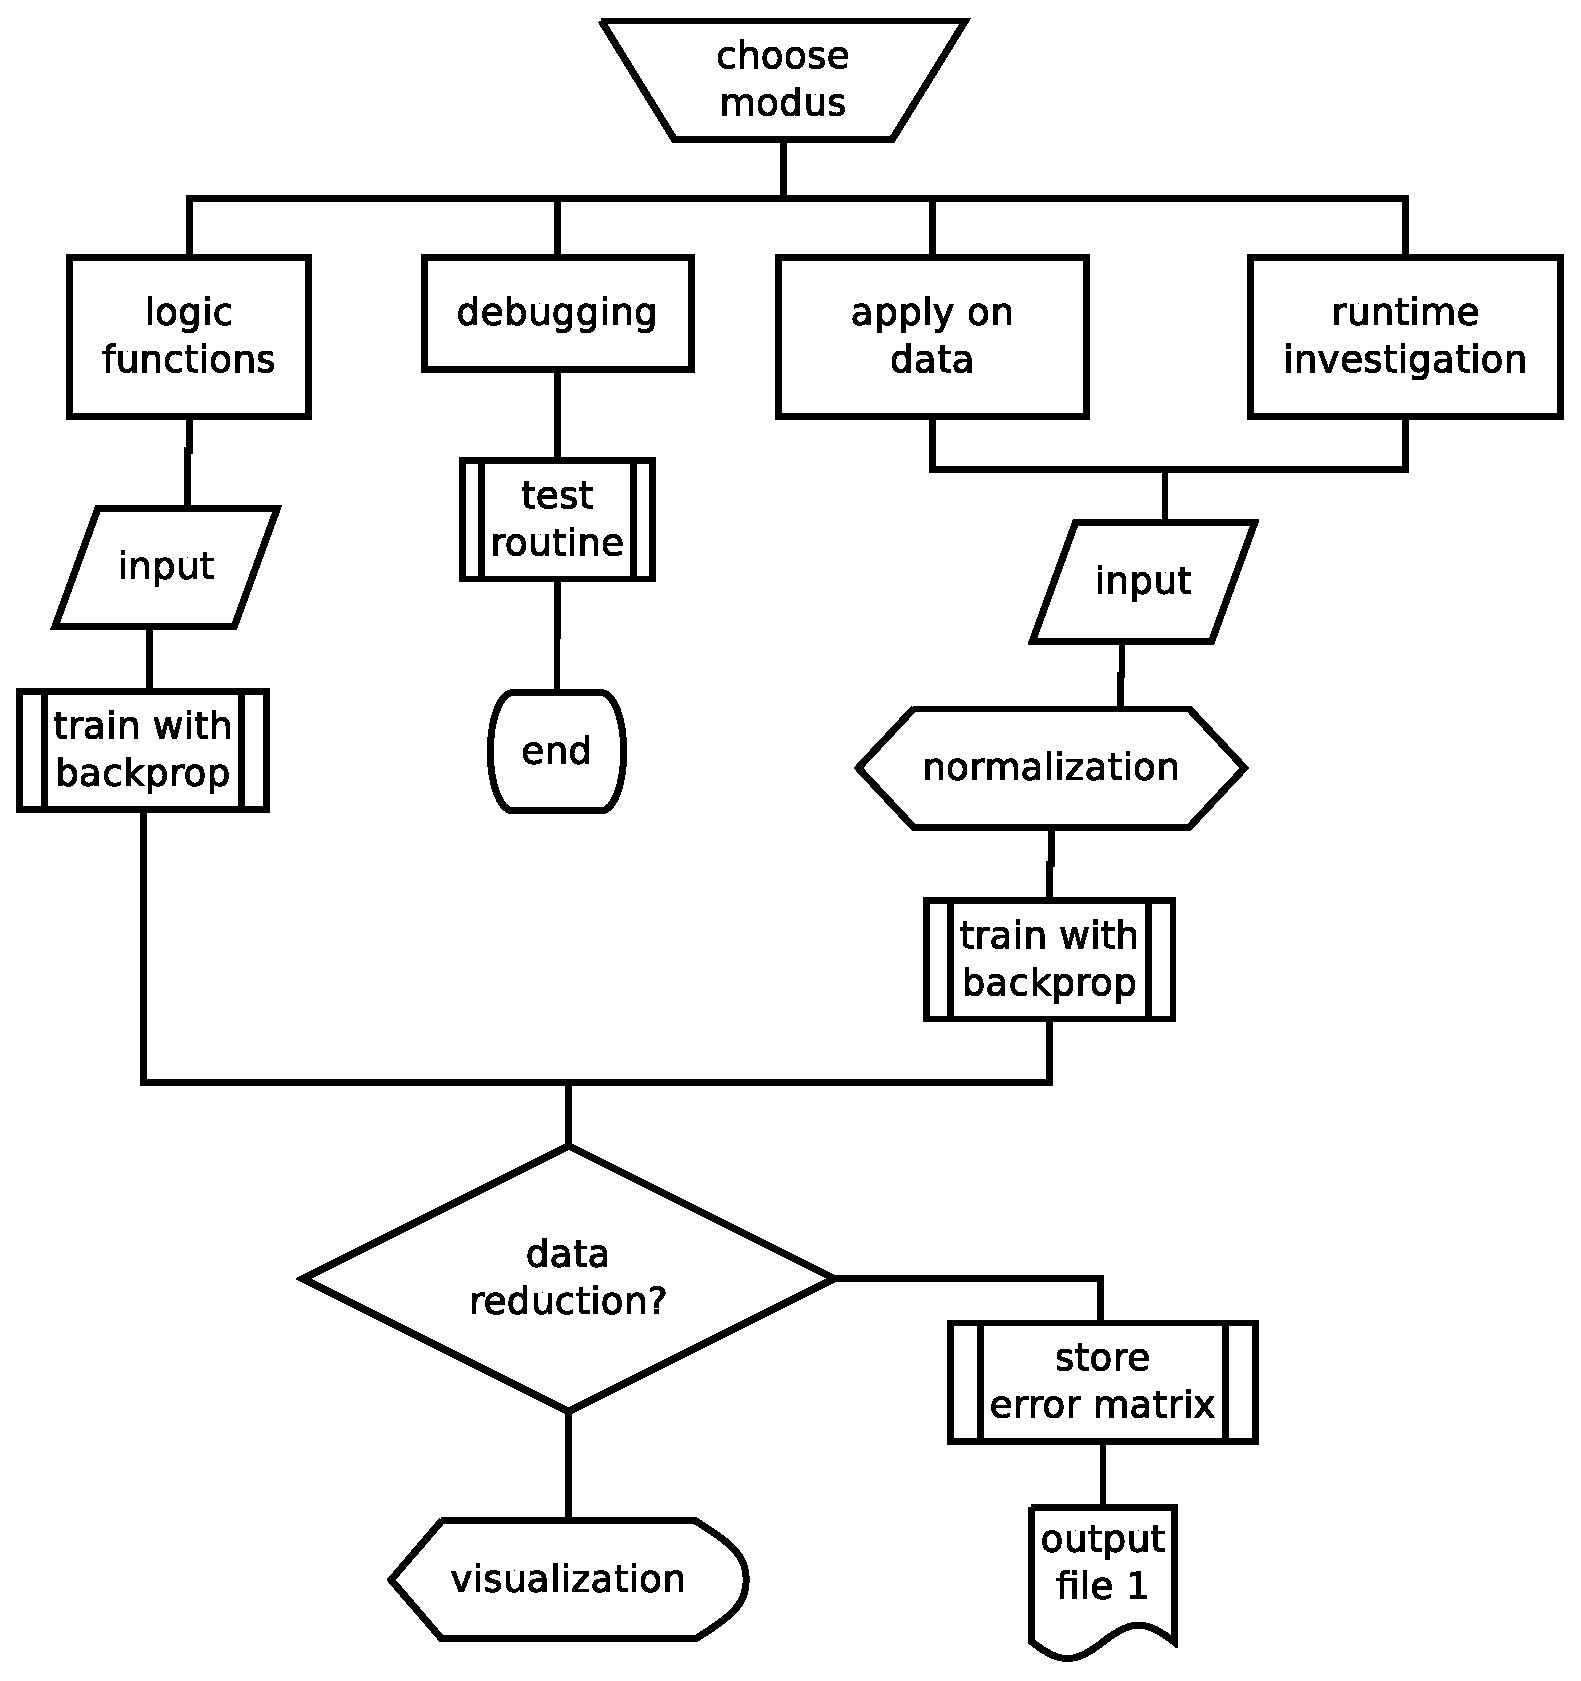
\includegraphics[width=6cm]{fig/dia.eps}
  \end{figure}

\end{frame}

\begin{frame}
  \frametitle{Input}
  \begin{eqnarray*}
    \mathbf{r}_i' &=& \mathbf{r}_i-\tilde{\mathbf{r}},\\
    \mathbf{r}_i''&=& \mathbf{s}\cdot\mathbf{r}_i',\\
    \mathbf{e}_i''&=& \mathbf{s}\cdot\mathbf{e}_i',
  \end{eqnarray*}
  \begin{table}
    \begin{center}
      \begin{tabular}{|lcl|lcl|}\hline
        original&&&normalized&&\\
        \hline\hline
        ( 6.7,49.6)&$\pm$&(1.7,2.5) & (0.0,0.4)&$\pm$&(0.02,0.02)\\
        (46.6,69.8)&$\pm$&(2.7,2.9) & (0.4,0.6)&$\pm$&(0.03,0.03)\\
        (93.5,20.2)&$\pm$&(1.6,3.3) & (1.0,0.1)&$\pm$&(0.01,0.03)\\
        (58.5,96.2)&$\pm$&(4.7,0.8) & (0.5,1.0)&$\pm$&(0.05,0.00)\\
        (23.7,10.0)&$\pm$&(2.5,2.8) & (0.1,0.0)&$\pm$&(0.02,0.03)\\
        $\ldots$   &$\pm$&$\ldots$  & $\ldots$ &$\pm$&$\ldots$\\
        \hline
      \end{tabular}
    \end{center}
  \end{table}
\end{frame}

\begin{frame}
  \frametitle{Training}
  \texttt{void \textbf{train}(int nitmax, double a, double eta) \{}

  \texttt{\qquad for (int nit = 0; nit < nitmax; ++nit) \{}

  \texttt{\qquad\qquad int i = (ttout.size() * Math.random());}

  \texttt{\qquad\qquad setInput(ttin.elementAt(i));}

  \texttt{\qquad\qquad setTarget(ttout.elementAt(i));}

  \vspace{0.2cm}

  \texttt{\qquad\qquad \textbf{fireCascade(a);}}

  \texttt{\qquad\qquad \textbf{getErr();}}

  \texttt{\qquad\qquad \textbf{correctW(eta);}}

  \texttt{\qquad\}}

  \texttt{\}}

\end{frame}

\begin{frame}
  \frametitle{findFunction}
  \texttt{@Override public SFunction \textbf{findFunction}() \{}

  \texttt{\qquad double a = 0.2, eta = 0.9;}

  \texttt{\qquad int nitmax = 10000;}

  \texttt{\qquad \textbf{generateTraining();}}

  \texttt{\qquad \textbf{n.train(nitmax, a, eta);}}

  \texttt{\qquad n.setInput( in );}

  \texttt{\qquad Matrix fin = new Matrix(\textbf{n.fireCascade(a)});}

  \texttt{\qquad double type = fin.get(0, 0) * 6.0;}

  \texttt{\qquad double deg = fin.get(1, 0) * 4.0;}

  \texttt{\qquad return new SFunction(type, deg);}

  \texttt{\}}

\end{frame}

\section{Output}
% \subsection{overview}
\begin{frame}
  \tableofcontents
\end{frame}

\subsection{Logic Functions on Two Input Neurons $(a,b)$}
\begin{frame}
%  \frametitle{Logic Functions}

  \begin{table}
    \begin{tabular}{|cccc|l|}\hline
      $(0,0)$&$(0,1)$&$(1,0)$&$(1,1)$&error $e$\\
      \hline\hline
      0 & 0 & 0 & 0 & 0.0000\\
      1 & 0 & 0 & 0 & 0.0005\\
      $\ldots$&&&&\\
      1 & 0 & 1 & 0 & 0.0003\\
      0 & 1 & 1 & 0 & {\bf 0.0021}\\
      1 & 1 & 1 & 0 & 0.0007\\
      0 & 0 & 0 & 1 & 0.0009\\
      1 & 0 & 0 & 1 & {\bf 0.0010}\\
      0 & 1 & 0 & 1 & 0.0004\\
      $\ldots$&&&&\\
      0 & 1 & 1 & 1 & 0.0006\\
      1 & 1 & 1 & 1 & 0.0000\\
      \hline
    \end{tabular}
  \end{table}

\end{frame}

\subsection{Output Window}
\begin{frame}
%  \frametitle{Output Window}
  \begin{figure}
    \centering
    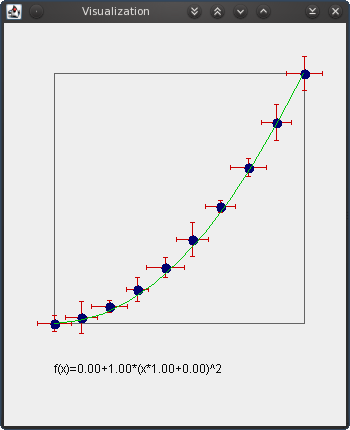
\includegraphics[height=0.8\textheight]{fig/vis.png}
  \end{figure}
\end{frame}

\subsection{Applied on Training Data}
\begin{frame}
%  \frametitle{applied on Training Data}
\begin{columns}
  \column{0.5\textwidth}
  \begin{table}
    \begin{tabular}{|ll|ll|}\hline
      type&deg&found&\\
      \hline\hline
      1 & 1 & 0.968 & 1.018 \\
      1 & 2 & 1.000 & 2.022 \\
      1 & 3 & 1.024 & 3.035 \\
      1 & 4 & 1.019 & 3.982 \\
      \hline
      2 & 1 & 2.003 & 1.016 \\
      2 & 2 & 2.019 & 2.012 \\
      2 & 3 & 1.983 & 2.989 \\
      2 & 4 & 2.010 & 3.938 \\
      \hline
      3 & 1 & 2.955 & 1.041 \\
      3 & 2 & 3.039 & 2.008 \\
      3 & 3 & 2.972 & 3.029 \\
      3 & 4 & 3.029 & 3.901 \\
      \hline
    \end{tabular}
  \end{table}
  \column{0.5\textwidth}
  \begin{table}
    \begin{tabular}{|ll|ll|}\hline
      type&deg&found&\\
      \hline\hline
      4 & $1\ldots4$ & {\bf 4.001} & {\bf 2.587} \\
      \hline
      5 & 1 & 5.010 & 1.075 \\
      5 & 2 & 5.026 & 2.065 \\
      5 & 3 & 4.997 & 3.086 \\
      5 & 4 & 4.991 & 3.974 \\
      \hline
      6 & 1 & 5.906 & 1.077 \\
      6 & 2 & 5.965 & 2.089 \\
      6 & 3 & 5.974 & 3.061 \\
      6 & 4 & 5.938 & 3.946 \\
      \hline
    \end{tabular}
  \end{table}
\end{columns}
\end{frame}

\subsection{Applied on Noisy Data}
\begin{frame}
%  \frametitle{Noisy Data}
  \begin{figure}
    \begin{center}
      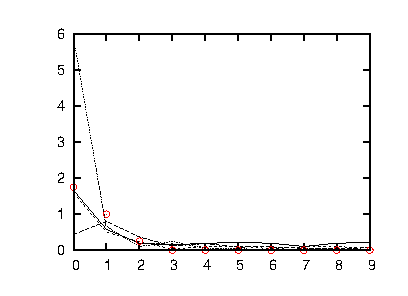
\includegraphics[width=3.5cm]{fig/err/ea1.eps}
      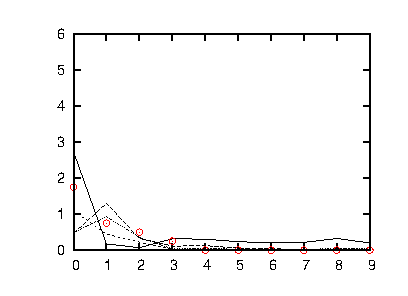
\includegraphics[width=3.5cm]{fig/err/ea2.eps}
      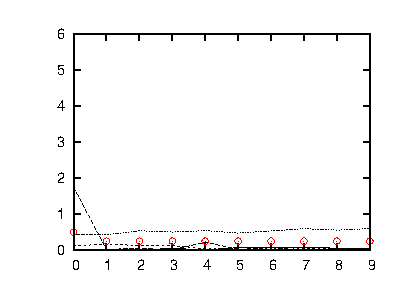
\includegraphics[width=3.5cm]{fig/err/ea3.eps}
    \end{center}
    \begin{center}
      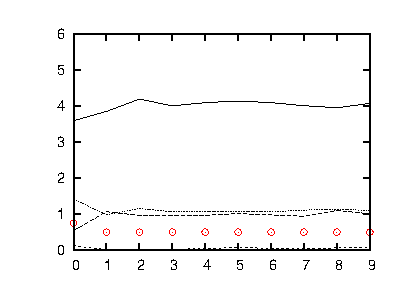
\includegraphics[width=3.5cm]{fig/err/ea4.eps}
      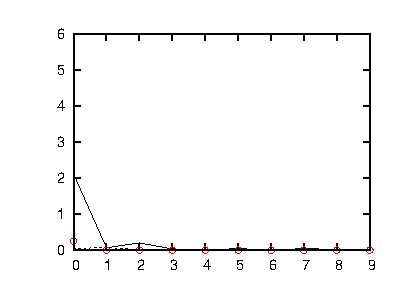
\includegraphics[width=3.5cm]{fig/err/ea5.eps}
      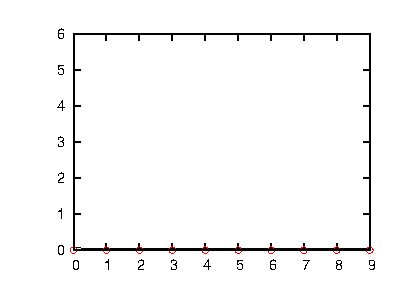
\includegraphics[width=3.5cm]{fig/err/ea6.eps}
    \end{center}
  \end{figure}
  \begin{equation*}
    10(1-\delta)\%
  \end{equation*}
\end{frame}

\section{Errors}
%\subsection{overview}
\begin{frame}
    \tableofcontents
\end{frame}
\subsection{Parametrization of Sigmoid Function}
\begin{frame}
  % \frametitle{as Function of Sigmoid Function}
  \begin{eqnarray*}
    {\rm sig}_a(x)&\equiv&\frac{1}{1+\exp(-ax)}\\
    {\rm sig}'_a(x)&=&a\cdot{\rm sig}_a(x)[1-{\rm sig}_a(x)]
  \end{eqnarray*}
  \begin{figure}
    \centering
    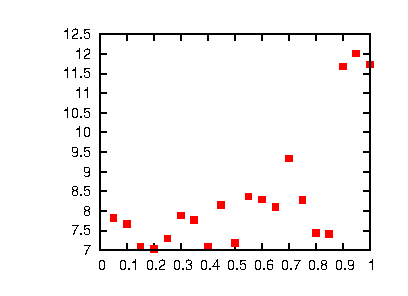
\includegraphics[width=5cm]{fig/err/ea.eps}
  \end{figure}
\end{frame}

\subsection{Learning Rate, Number of Iterations}
\begin{frame}
%\frametitle{as Function $n_{it},\eta$}
	\begin{figure}
		\centering
		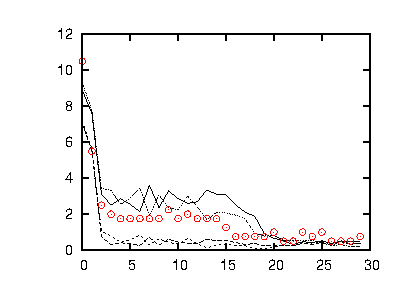
\includegraphics[width=3.5cm]{fig/err/e1.eps}
		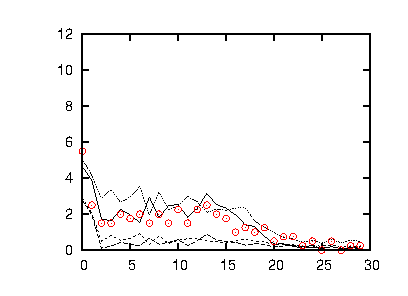
\includegraphics[width=3.5cm]{fig/err/e2.eps}
		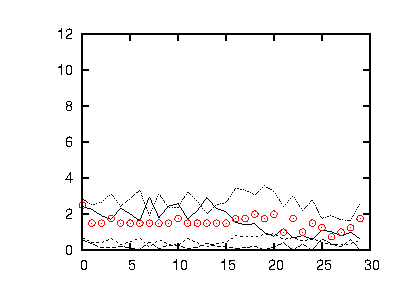
\includegraphics[width=3.5cm]{fig/err/e3.eps}
	\end{figure}
	\begin{figure}
		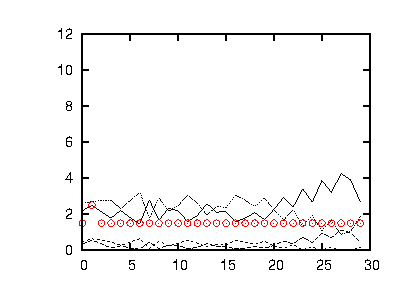
\includegraphics[width=3.5cm]{fig/err/e4.eps}
		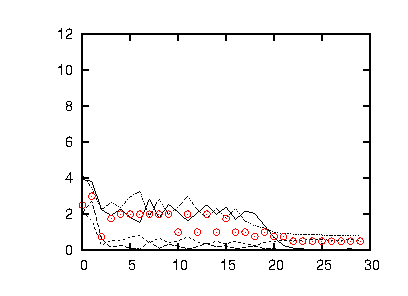
\includegraphics[width=3.5cm]{fig/err/e5.eps}
		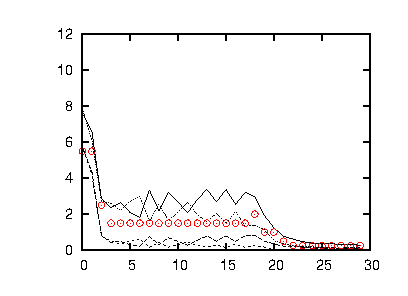
\includegraphics[width=3.5cm]{fig/err/e6.eps}
	\end{figure}
        \begin{equation*}
          \cdot1000
        \end{equation*}
\end{frame}

\subsection{Number of Hidden Neurons}
\begin{frame}
%\frametitle{as Function \#Neurons}
\begin{table}
\begin{tabular}{|r|r|r|}\hline
$n_{{\rm hid,(1,2)}}$&error&time $[{\rm s}]$\\
\hline\hline
 1&86.23& 1.7\\
 2&30.56& 1.9\\
 3&14.84& 2.5\\
 4&12.38& 2.9\\
 5& 9.31& 3.5\\
 6&10.79& 4.0\\
 7&10.00& 4.7\\
 8& 9.32& 5.3\\
 9& 9.33& 6.0\\
10& 7.32& 6.7\\
\hline
15& 7.64&11.3\\
\hline
20& 6.58&17.5\\
\hline
\end{tabular}
\end{table}

\end{frame}

\section{To Be Done}
\subsection{Projects}
\begin{frame}
\begin{itemize}
  \item more sampling points
  \item random input
  \item linear superposition
  \item three-dimensional data
  \item holographic neuron (with 2D FFT)
  \item ...
\end{itemize}

\end{frame}

\end{document}
